\documentclass[12pt]{article}
\usepackage{ctex} %latex写中文文章时的包
\usepackage{geometry}%公式对齐,设置版面工具包
\usepackage{graphicx}%插入图片的宏包
\graphicspath{}%确认图像文件夹路径
\usepackage{amsmath}%公式对齐的工具包,效果看公式(2)
\usepackage{indentfirst}%首行缩进包
\usepackage{caption}
\usepackage{subfigure}
\geometry{left=2.8cm,right=2.8cm,top=2.54cm,bottom=2.54cm}
\title{Python Final Homework}
\author{Botong Zhao ID:201928013919007}

\begin{document}
	\maketitle
	\begin{abstract}
		作为python课程的最后一次作业,也是第一次python项目作业。本项目主要分为三个部分:1,对长春光机所新闻网(http://www.ciomp.ac.cn/xwdt/zhxw/)的信息进行爬虫收集并进行分类;2对新闻数据简单处理后进行数据分析并画图;3将爬取的文本信息制作成wordcloud。
		经过整理:其结果为2016年9月-2019年11月1日一共有新闻1000条,共1139天,163周,平均每天新闻0.878条,每周新闻平均6.13条。
	\end{abstract}
	\section{爬虫处理}
	本爬虫程序的结构分为两个文本,第一个文本是函数库FunctionFile.py。用于对调用的函数库和以及建立的函数进行汇总,方便主程序运行并且看起来更加简洁。另外在程序中插入多个print节点(已注释取消)用于检查输出的结果是否正确(属于个人习惯)。下面对爬虫程序进行说明。
	\subsection{Get The Dataset By Beautifulsoup}
	首先将FunctionFile.py文件进行导入并as为FF函数,方便调用。定义要爬取网页的url,这里我们的url为长春光机所综合新闻网"http://www.ciomp.ac.cn/xwdt/zhxw/index.html"以字符串的形式定义,放入FF.openTheWeb(url)获取html。之后使用BeautifulSoup对html进行解析,解析工具为"html.parser",获取soup。完成解释后调用语法:
	
	$$
	title=soup.find_all('a',class_="font06")
	date=soup.find_all('td',class_= "riqi")
	$$
	
	找到目标标题和日期对应的class并进行信息爬取储存。这时打开一个txt文本中作为方便阅读的新闻目录。之后调用函数FF.crawlerSubPage(info,title,date,output1),爬取每个标题的新闻,每爬取一个新闻的内容便创建一个新的txt文本用于储存新闻主体,将日期和标题作为txt文件名并写在之前定义好的txt目录中。
	
	当我们爬取成功第一页后发现第2页到第37页的url地址每一页都不同,这个时候借助一个for函数循环爬取每一页的新闻标题,日期以及新闻主体(此处的print是为了检查爬取的url地址是否正确如果正确则注释取消)。在爬取所有的新闻之后关闭目录的txt文本并保存。
	\subsection{open the web}
	此函数的作用为获取页面的源码用于下一步爬虫提取信息。注释掉的信息是为了检查是否成功提取出正确的网页源码。如果提取源码成功则返回结果用作下一步BeautifulSoup分析。
	
	\subsection{text creat}
	
	用于保存爬取的每一条新闻主体并存储在message文件夹下,输入为想要保存的新闻标题及日期作为txt文件的文件名。之后将txt文件打开,写入新闻主体,关闭并保存txt文件。
	其效果如下图所示。
	\begin{figure*}[htb]
		\centering
		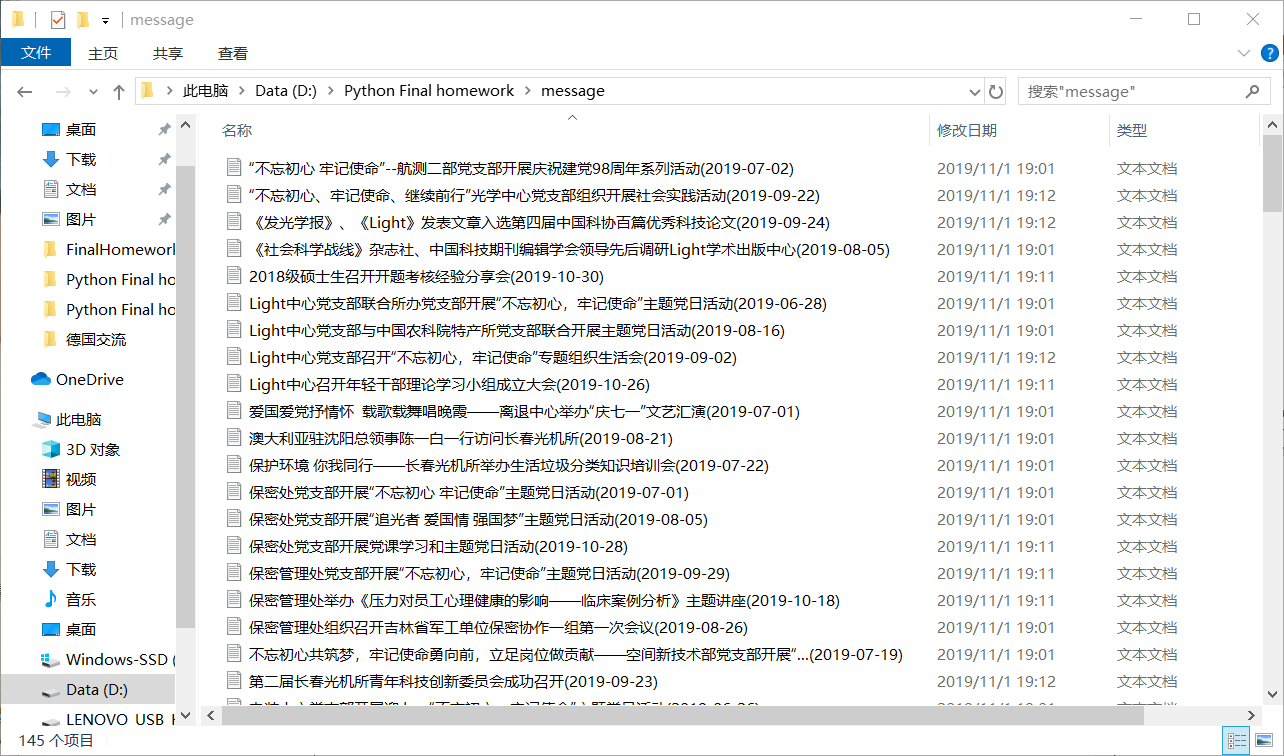
\includegraphics[scale=0.35]{message.png}
		\caption{message文件夹——用于储存新闻}
	\end{figure*}

	\begin{figure*}[htb]
		\centering
		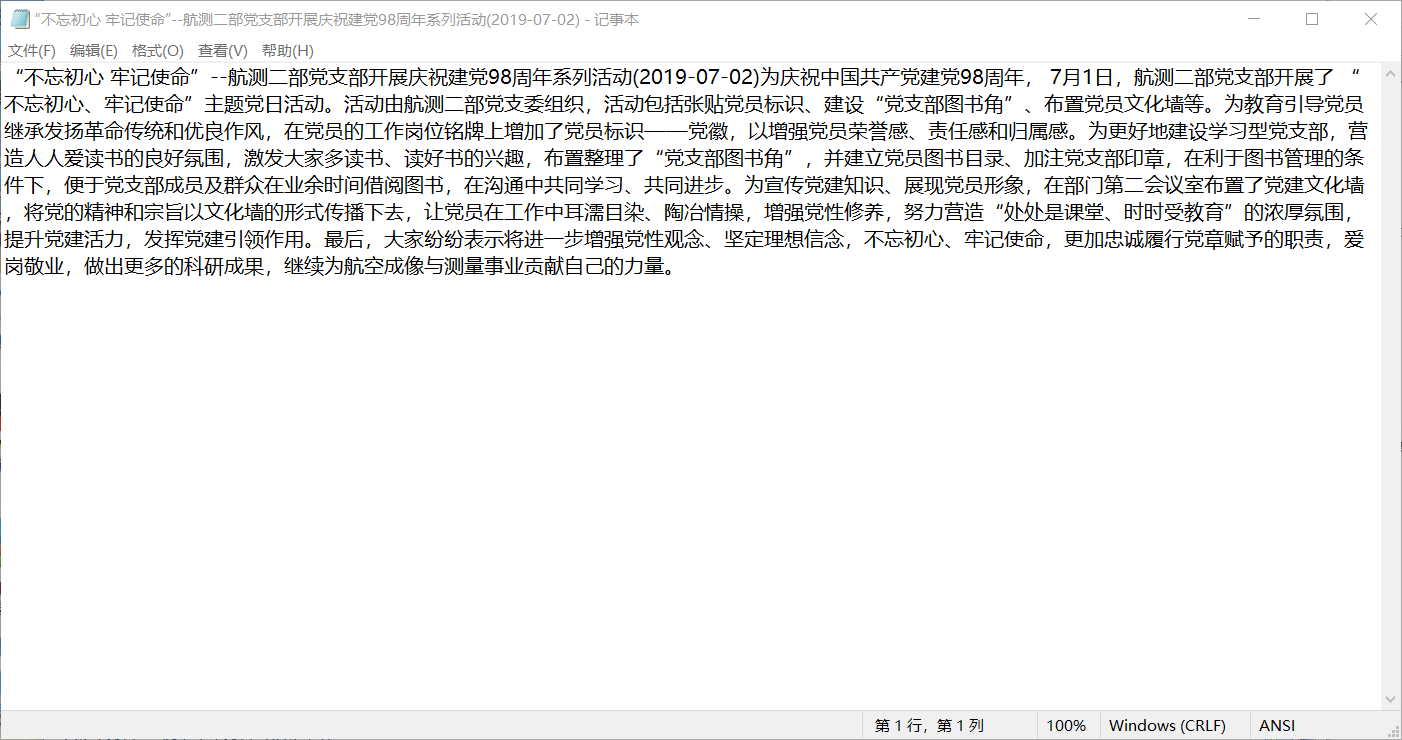
\includegraphics[scale=0.35]{news.png}
		\caption{新闻标题.txt——用于存储新闻主体}
	\end{figure*}

	\subsection{crawler Subpage}
	首先通过对源码分析获取标题的超链接,并对超链接进行访问,之后对访问后的子网页进行爬虫获取新闻主体。调用text creat函数创建文档对新闻进行保存,并将标题,时间和撰写部门命名为文件名以及写入dataset.txt文件用于下一步数据分析。
	
	\section{数据分析}
	\begin{figure*}[htb]
		
		\centering
		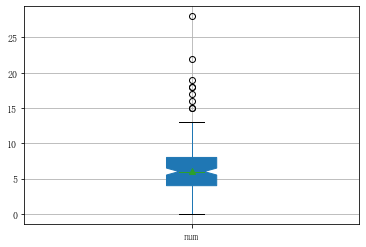
\includegraphics[scale=0.6]{boxplot.png}
		\caption{每周新闻的数量的boxplot}
	\end{figure*}
	当我们获取所有的新闻之后我们的数据分析并不需要新闻的主体,只需要对日期进行处理,这里我们使用的numpy函数库用于对DataFrame变量进行处理,并通过pandas对文件进行处理,最后再使用matlplotlib.pyplot生成我们的统计结果效果图
	
	在导入函数库之后,首先打开data获取数据定义为df,并对数据进行分类,借助$pd.to_dataset()$将获取的日期转化为日期形式,并且设置为index。

	之后借助$np.size(df,0)$获取所有的新闻总量,借助pandas对日期类型数据处理的能力进行统计,使用$df.resample('w').sum()$获得每一周的新闻总量,并且借助$plt.plot(week)$将每一周的新闻总数以曲线的形式展现。并生成为csv文件进行保存。
	

	计算平均每周和每天的新闻数记录之后记录,为了观察每周新闻数量的分布趋势,使用boxplot函数显示boxplot并对图片进行保存。
	\begin{figure*}[htb]
			\centering
			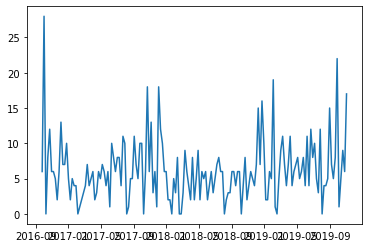
\includegraphics[scale=0.6]{eachweeknews.png}
			\caption{每周新闻的数量}
	\end{figure*}

	\section{wordcloud}
	WordCloud 是一款python环境下的词云图工具包,同时支持python2和python3,能通过代码的形式把关键词数据转换成直观且有趣的图文模式。这里我们会使用jieba和wordcloud里面的WordCloud, STOPWORDS, ImageColorGenerator。并且使用matplotlib.pyplot生成词云图片。
	
	在定义stopword的函数中首先使用jieba.cut返回一个迭代器$word_generator$,打开$stop word.txt$。并且读取$stopword$,需要注意的是$stop word$的格式是一词一行,之后将word generator里面的每个词进行循环添加到$word_list$里面.
	
	载入并解析一个图片,调用worldcloud函数并设置参数。打开数据集文件,载入stopword函数中得到stop word list,并利用$jieba.load_userdict()$载入NoCut.txt'。之后使用$wc.generate(wc)$生成词云,并且基于彩色图片生成相应彩色单词和词云轮廓。再使用plt展示词云图片并保存。
	
	\begin{figure*}[htb]
		\centering
		
\includegraphics[scale=0.3]{WordCloud.png}
		\caption{词云}
	\end{figure*}

	\section{总结}
	首先很庆幸自己选到了这门个性化选修课,可能是我个人比较认为这门课程所用的语言很特别很奇妙,老师也很有趣,能让我们更好的了解Python这门课程真正的用途。在学习Python这门课程的这段时间以来,并且自己也能认识并且学习到很多知识。
	
	非常感谢老师,帮助我及时复习了python的基础知识,并且第一次学习了爬虫,非常有趣。希望结课以后也可以继续和老师交流学习,谢谢老师。
\end{document}